\chapter{Benchmark}
In questo breve capitolo verranno mostrati
alcuni risultati di \pygfa \  evidenziando il tempo di calcolo
richiesto per alcune delle operazioni che la libreria fornisce e misurando
lo spazio di memoria richiesto per l'immagazzinamento del grafo.
Verranno infine presentati dei grafici che evidenziano il
confronto con la libreria Gfapy in termini di tempo di esecuzione
e di spazio occupato.

Tutte le operazioni sono state effettuate su una macchina virtuale
Linux 64bit con le seguenti caratteristiche:
\begin{itemize}
	\item \SI{8}{\giga\byte} di ram;
	\item processore host da \SI{3.7}{\giga\hertz} quad-core, il
		sistema guest sfrutta due soli core;
	\item hard disk magnetico.
\end{itemize}

Le misure sono state effettuate su grafi generati casualmente
da uno script usato nello sviluppo di Gfapy; il programma
crea una serie di nodi collegati tra loro da sovrapposizioni
a coda di rondine, il risultato viene salvato in un file GFA1.
Visto che i grafi sono generati casualmente è improbabile
che si riesca a ripresentare la stessa configurazione di componenti
connesse e sequenze di unitig (a meno di salvare i file generati),
mentre il numero di nodi e archi rimane prestabilito al ripetersi
dei test. Per \emph{elementi del grafo}, nel contesto dei grafici presentati,
si intendono l'insieme di nodi e archi del grafo.
Per automatizzare la misurazione delle performance è stato
scritto un programma che si occupa di generare automaticamente
i grafi, effettuare le misurazioni, salvare i risultati su un file di testo
e rimuovere i grafi creati al termine.

Le operazioni che si sono andate a misurare sono:
\begin{itemize}
	\item il tempo impiegato per effettuare il parsing del file contenente il grafo;
	\item il tempo richiesto per ottenere i dizionari contenenti i nodi e gli archi;
	\item il tempo per calcolare le componenti connesse (sia considerando
		solo archi di dovetail sia considerando tutti i tipi di archi)
		\footnote{In questo caso, visto che lo script genera solo archi a coda
		di rondine, le componenti connesse individuate saranno le medesime. Si tenga
		comunque a mente che il tempo misurato riguarda il calcolo di entrambi
		i tipi di componenti connesse.};
	\item il tempo richiesto per la ricerca delle sequenze di unitig.
\end{itemize}
Oltre alla misura di questi tempi si è andato a misurare il consumo
di memoria necessario per contenere il grafo GFA.
\clearpage

\captionsetup{justification=centering, singlelinecheck=false}
\begin{figure}[h]
\centering
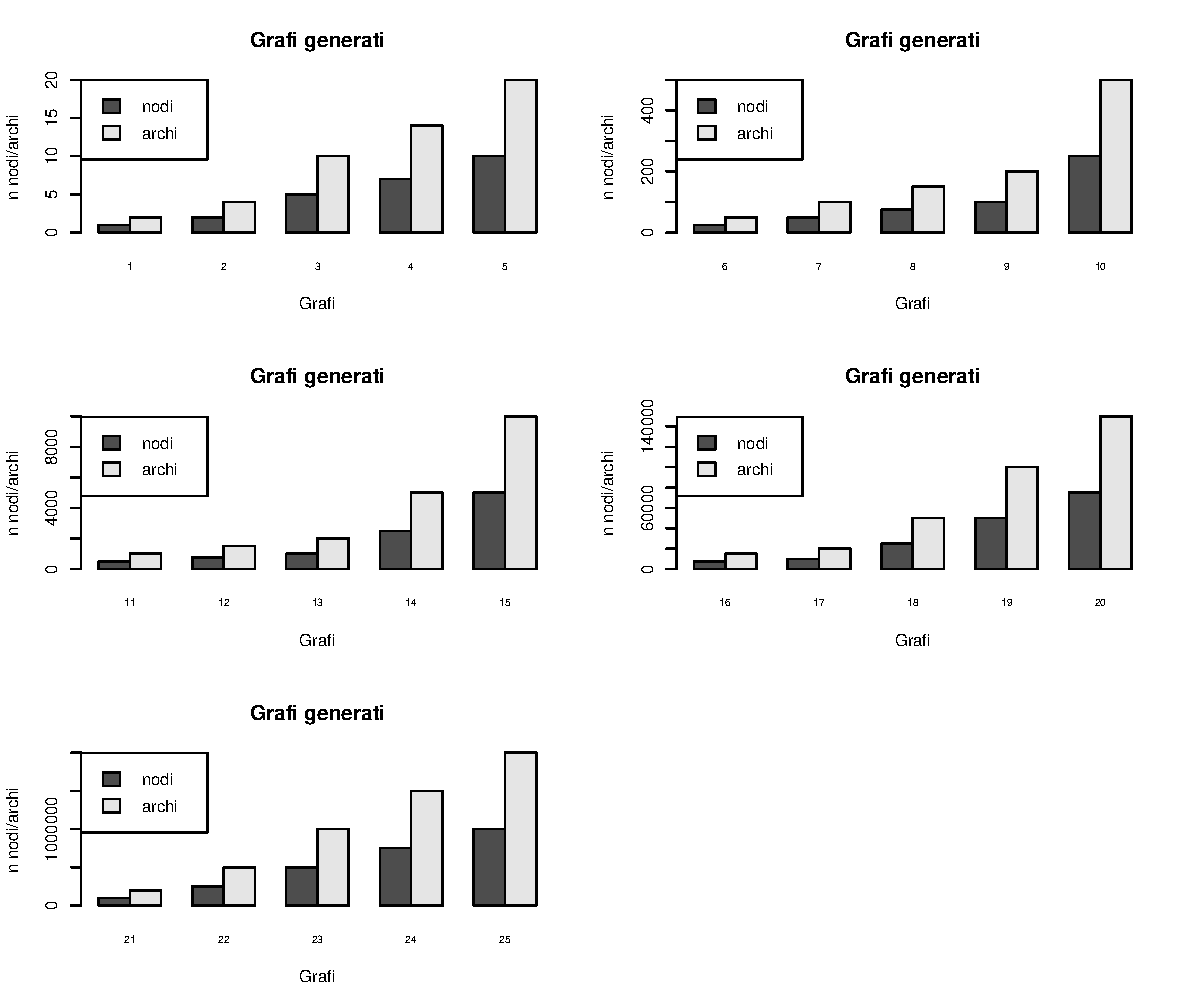
\includegraphics[scale=0.75]{benchmark_grafi}
\caption[Grafico a barre dei grafi generati]{Grafici a barre relativi i numeri di nodi e archi dei grafi generati.}
\end{figure}
\captionsetup{justification=justified, singlelinecheck=false}
Per il numero dei nodi dei grafi generati si sono prese in considerazione
le potenze di dieci generando, all'aumentare dell'esponente, grafi il cui
numero di nodi ripercorreva i fattori 1, 2.5, 5, 7.5 e 10.
Si sono creati quindi 25 grafi, raggiungendo la soglia
del milione di nodi, collegati tra loro da due milioni di archi.


\captionsetup{justification=centering, singlelinecheck=false}
\begin{figure}
\centering
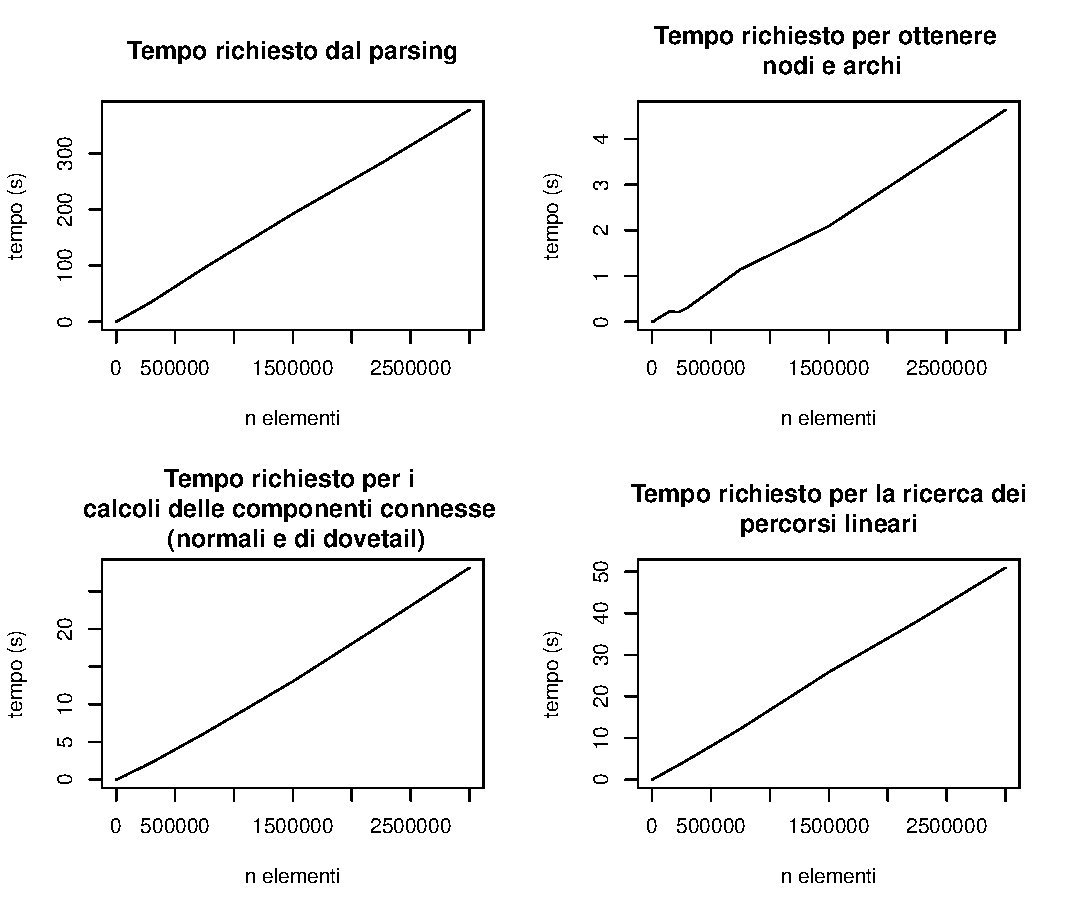
\includegraphics[scale=0.75]{benchmark_tempi}
\caption[Grafici dei tempi di calcolo delle operazioni su grafo]{Misurazioni dei tempi di calcolo.}
\label{fig:bench-timings}
\end{figure}
\captionsetup{justification=justified, singlelinecheck=false}
I tempi (figura \ref{fig:bench-timings}) indicano un andamento lineare
per tutte le operazioni eseguite. Il caso peggiore si ha nel caso
della funzione di ricerca delle sequenze di unitig, la quale
impiega un tempo doppio rispetto la ricerca delle componenti connesse.
I tempi per la lettura del file sono lineari e strettamente vincolati
dal tempo di accesso del supporto magnetico, si può pensare di ottenere
un risultato decisamente migliore usando un SSD, visto che
ha un tempo accesso più veloce.

\clearpage
\captionsetup{justification=centering, singlelinecheck=false}
\begin{figure}[h]
\centering
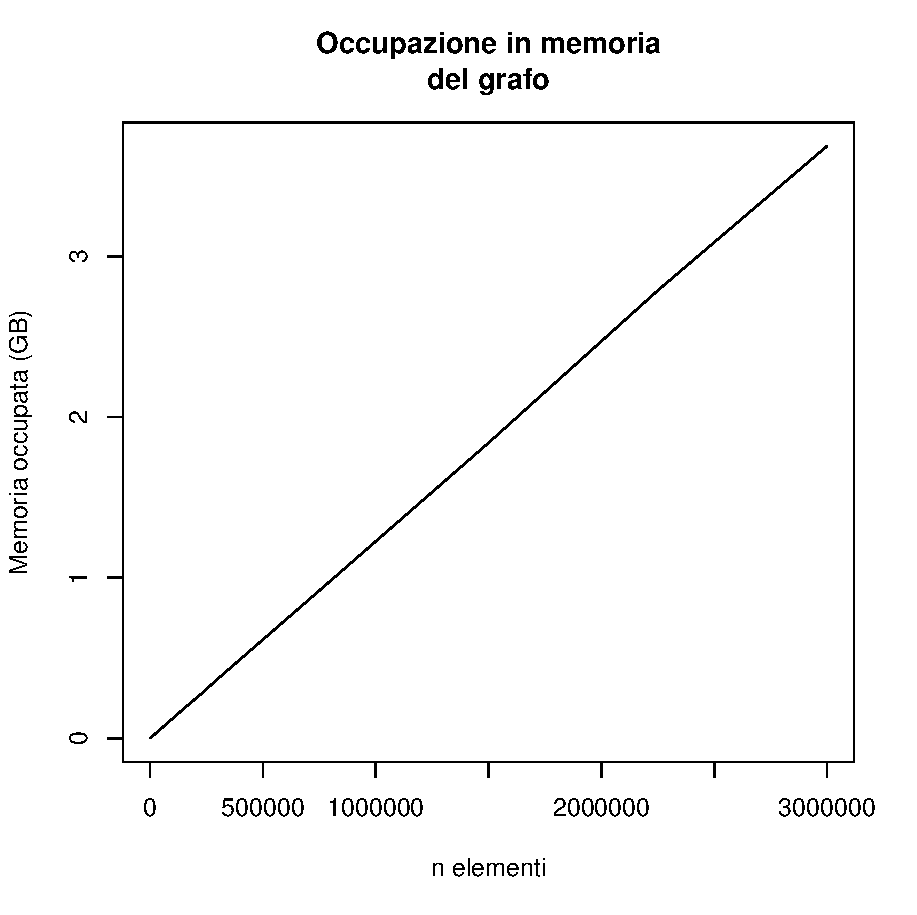
\includegraphics[scale=0.75]{benchmark_memoria}
\caption[Grafici della memoria occupata dal grafo]{Misurazione della memoria occupata dal grafo.}
\label{fig:graph-memory}
\end{figure}
\captionsetup{justification=justified, singlelinecheck=false}
L'uso della libreria NetworkX, come già accennato a pagina \pageref{sec:nx-why-limits},
comporta una grossa occupazione della memoria. I dati riportati nel grafico
in figura \ref{fig:graph-memory}
riguardano il peso del grafo GFA subito dopo la sua creazione da file, senza
prendere in considerazione la memoria di ``contesto'' necessaria per avviare
il processo Python e la libreria standard. In totale la memoria occupata
raggiungeva, nell'ultimo grafo, circa i \SI{4.2}{\giga\byte} raggiungendo
il limite di \SI{5.1}{\giga\byte} durante la ricerca dei percorsi lineari, operazione
che si è rivelata essere la più dispendiosa fra quelle misurate.

% Confronto Gfapy e PyGFA
\section{Confronto con Gfapy}
Nei seguenti grafici sono indicati i dati ottenuti eseguendo con le librerie
Gfapy e \pygfa le operazioni di parsing ed estrazione degli elementi del
grafo da un file gfa, estrazione dei dizionari contenenti le informazioni
del grafo e calcolo delle componenti connesse; mostrando
le differenze sia in termini di tempo di esecuzione (figura \ref{fig:comparison-times})
che di spazio occupato dal grafo (figura \ref{fig:comparison-memory}).

Per ottenere questi dati sono stati generati grafi casuali fino ad un limite massimo di cinquemila nodi
e diecimila archi. Tale limite è dovuto a delle problematiche riscontrate con l'uso di Gfapy
per grafi con numero di elementi maggiore, oltre il quale
l'operazione di calcolo delle componenti connesse causa problemi dovuti
probabilmente alla natura ricorsiva del metodo implementativo in Python.
Come evidenziato dai grafici, il tempo di esecuzione relativo il parsing
è maggiore in Gfapy, mentre il tempo richiesto per accedere ai dizionari
contenenti gli elementi del grafo è pressoché costante in entrambe le librerie.
Per quanto riguarda il calcolo delle componenti connesse \pygfa \ è nettamente
più veloce. Dall'ultimo grafico è possibile notare come il
consumo di memoria richiesto è all'incirca il medesimo.

\captionsetup{justification=centering, singlelinecheck=false}
\begin{figure}[h]
\centering
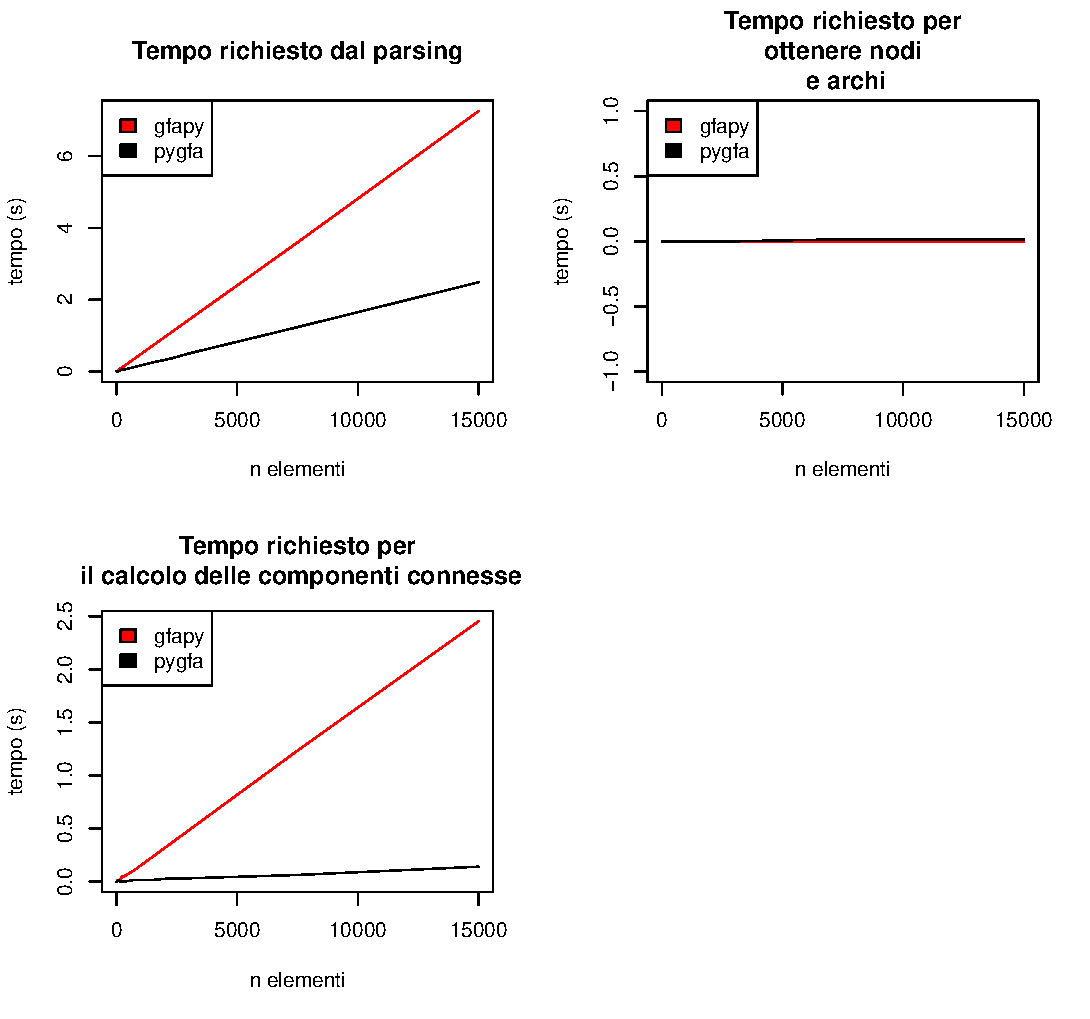
\includegraphics[scale=0.75]{comparison_times}
\caption[Grafici dei tempi di esecuzione di Gfapy e \pygfa]{Grafici dei tempi di esecuzione di Gfapy e \pygfa.}
\label{fig:comparison-times}
\end{figure}
\captionsetup{justification=justified, singlelinecheck=false}


\captionsetup{justification=centering, singlelinecheck=false}
\begin{figure}[h]
\centering
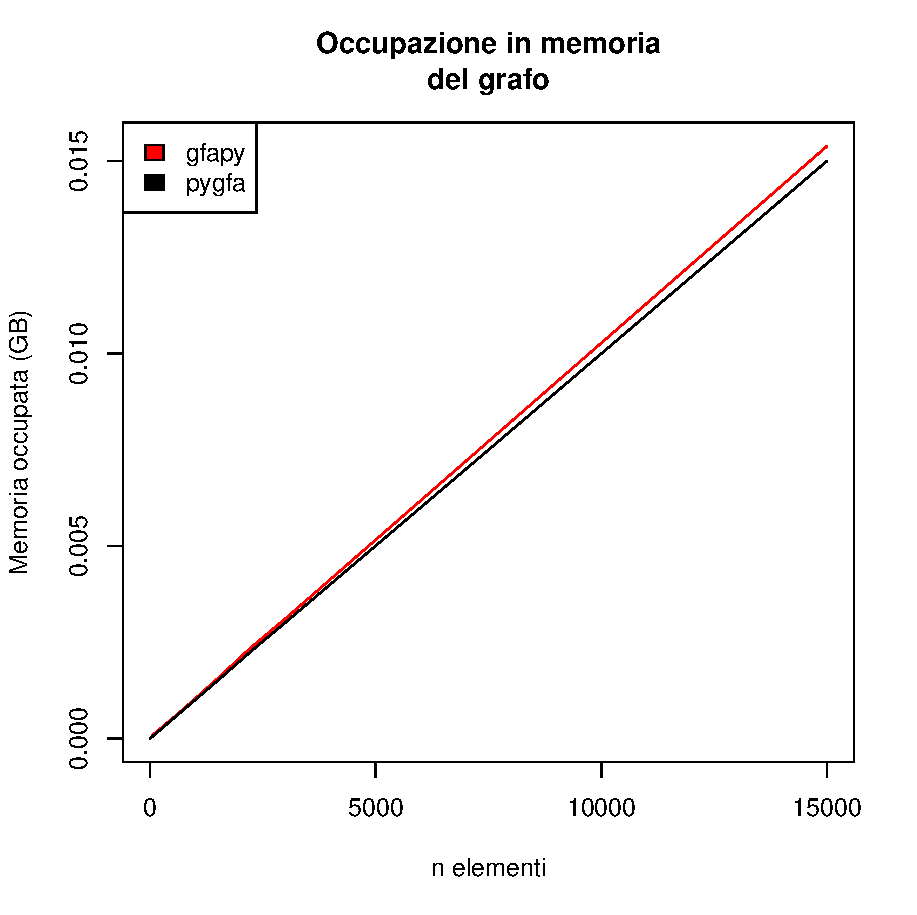
\includegraphics[scale=0.75]{comparison_memory}
\caption[Grafico della memoria usata da Gfapy e \pygfa]{Grafico della memoria usata da Gfapy e \pygfa.}
\label{fig:comparison-memory}
\end{figure}
\captionsetup{justification=justified, singlelinecheck=false}


\clearpage
\section{Conclusioni}
\pygfa \  ha gli stessi punti di forza e di debolezza di NetworkX:
le operazioni sono molto veloci, ma a costo della memoria occupata.
Nonostante ciò, la rapidità di sviluppo e l'ottima efficienza di questa libreria
rendono \pygfa \  un sistema performante molto facile da ampliare e modificare.
Messo a confronto con Gfapy, la libreria riesce ad eseguire alcune operazioni
in tempi decisamente migliori a parità di occupazione in memoria.
